\documentclass[a4paper,11pt,twoside]{report}%pridat twoside, do [] pre obojstrannu tlac
    \pagestyle{headings}
    \usepackage[top=2.5cm, bottom=2.5cm, left=3.5cm, right=2cm]{geometry} %odporucane okraje

\usepackage[utf8x]{inputenc}
\usepackage[T1]{fontenc} %pekne makcene
\usepackage{algorithmic}
\usepackage{algorithm}
\usepackage{amsmath}
\usepackage{amssymb}
\usepackage{graphicx}
\usepackage{graphics}
\usepackage{cite}

\graphicspath{ {pictures/} }
\renewcommand{\thesection}{\arabic{section}}

\author{Matus Behun}
\title{Cayley graphs of given diameter on linear groups}

\usepackage{hyperref}
    \hypersetup{colorlinks,citecolor=red,filecolor=black,linkcolor=blue,urlcolor=blue,pdftex}

\begin{document}
\setlength{\belowdisplayskip}{7pt} \setlength{\belowdisplayshortskip}{5pt}
\setlength{\abovedisplayskip}{7pt} \setlength{\abovedisplayshortskip}{5pt}

%====================================================================================================================================================
% FIRST PAGE 
%====================================================================================================================================================
\thispagestyle{empty}
{
	\topmargin=0pt
	\centerline {\large \bf{SLOVAK UNIVERSITY OF TECHNOLOGY}}
	\vskip 0.2cm
	\centerline{\large \bf{FACULTY OF CIVIL ENGINEERING}}
	\vskip 5cm
	\centerline{\Large \bf{Cayley's graph of given diameter on linear groups}}
	\vskip 0.2cm
	%\centerline{\Large \bf{HÝ JEHO DRUHÝ RIADOK}}
	%\centerline{ \bf{(verzia z~\today) }}   %vypisovanie dnesneho datumu
	\vskip 0.5cm
	\centerline{\large \bf{Bachelor's thesis}}
	\vskip 5cm          %\vskip 2cm             %zmena kvoli zobrazovaniu dnesneho datumu
	\normalsize
		\begin{tabular}[l]{p{0.27\textwidth}p{0.73\textwidth}}
		Študijny program: & Matematicko-počítačové modelovanie\\
		Študijny odbor: & Aplikovaná matematika\\
		Školiace pracovisko: & doplň ma\\
		Vedúci diplomovej práce: & doplň ma \\
		\end{tabular}
	\vskip 3cm
	\centerline{\large \bf{BRATISLAVA 2018}}
	\vskip 0.2cm
	\centerline{\large \bf{Matúš Behun}}
}

\pagebreak
\tableofcontents
\newpage

%====================================================================================================================================================
% END OF FIRST PAGE  
%====================================================================================================================================================

\section{Introduction}

Construction of network consisting of `nodes` as vertices and `links` between them as edges under certain graph topology properties can be difficult if possible. Restrictions for graph such as number of edges outgoing from node or \textit{degree} of vertices, length of path between any of them or \textit{diameter} or possibility to return by unwalked edges with certain path length or \textit{girth} of graph are examples. 

Making graph with biggest possible number of vertices while keeping degree and diameter is known as \textit{degree/diameter} problem and has been studied by many~\cite{Degree-diameter-survey}.

\newpage
%====================================================================================================================================================
% INTRODUCTION TO DEGREE DIAMETER PROBLEM ON UNDIRECTED GRAPHS strana 8, 9
%====================================================================================================================================================

\section{Degree/diameter problem}
\subsection{Moore bound}

There is theoretical upper bound named after Moore for order of graphs with given diameter $k$ and degree $d$. Bound is easily derived from construction of graph. Start with single vertex connected to $d$ vertices. Next step consists of making every of new $d$ vertices making adjacent to $d-1$ new vertices making them of degree $d$. There have to be $n$ such steps including first one to satisfy diameter restriction. 

\begin{equation}
	\begin{split}
		n_{d,k} \leq M_{d,k}	& = 1 + d + d(d - 1) + \dots + d(d - 1)^{k-1}  \\
				 				& = 1 + d(1 + (d - 1) + \dots + (d - 1)^{k-1}) \\
				 				& =	\begin{cases}
										1+d\frac{(d-1)^{k}-1}{d-2}, & \text{if}\ d > 2 \\
										2k+1, & \text{if}\ d=2 
									\end{cases}
	\end{split}
\end{equation}

%% About upper boundary
\subsection{Moore graphs}
In general $n_{d,k}$ in (1) equals to $M_{d,k}$ in few cases. Graphs with order equal $M_{d,k}$ are called by \textit{Moore} who first proposed problem of classifying there graphs~\cite{ Hoffman-Singleton }. Moore graphs are  necessary regular of degree $d$. Research of Moore graph was initiated by Hoffman and Singleton in paper~\cite{Hoffman-Singleton} with focus on diameter $2$ and $3$.They found Moore graphs with $k=2$ and $d=2,3,7$ which are unique and there is possibly graph with $d=57$ which hasn't been found yet. They also proved that for $k=3$ and $d=2$ heptagon is unique Moore graph. The proofs exploit eigenvalues and eigenvectors of the adjacency matrix (and its principal submatrices) of graphs. \\

Easily found Moore graphs for parameters $d=2$ and $k \geq 2$ are circle graphs $C_{2k+1}$, Moore graphs with diameter $k = 1$ and degree $d \geq 1$ are complete graphs $K_{d+1}$. Unique Moore graph for $n_{3,2}$ is Petersen graph and for $n_{7,2}$ Hoffman-Singleton graph.

\begin{figure}[!ht]
	\centering
	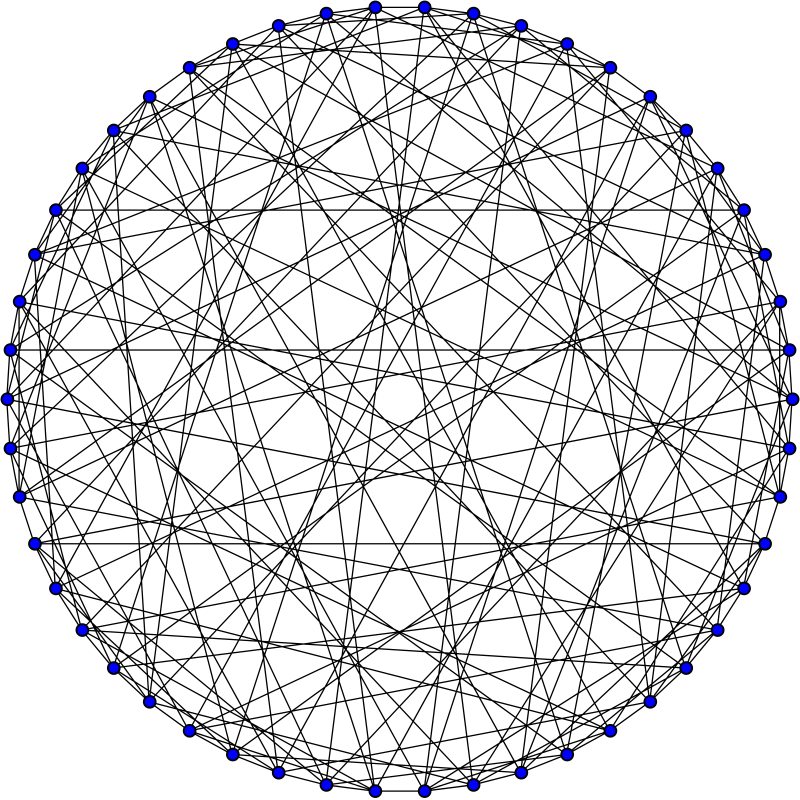
\includegraphics[scale=0.33]{Hoffman-Singleton_graph.png}
	\caption{Hoffman-singleton graph is Moore graph with $d=7$ and $k=2$ }
\end{figure}

%====================================================================================================================================================
% END OF INTRODUCTION TO DEGREE DIAMETER PROBLEM
%====================================================================================================================================================

%====================================================================================================================================================
% GRAPHS NON MOORE'S  
%====================================================================================================================================================

\subsection{Graphs close to Moore boundary}
Because there are only few graphs that satisfy theoretical Moore boundary there has been effort making graphs as close to it as possible. Graph with defect is denoted by $(d,k,-\delta)$ equal to graph of order $M_{d,k}-\delta$. Conventionally $\delta$ refers to small defect $\delta \leq d$ . 

Research yields many results concerning graph with defects. Erdős, Fajtlowitcz and Hoffman proved~\cite{Erdos-Fajtlowicz-Hoffman} that there is no graph of degree $d$ and diameter $2$ and $\delta = 1$ apart from cycle $C_{4}$.  
In case of  $\delta = 2$ with $d = 2$ are all $(d,k,-2)$ graphs cycles $C_{2k-1}$. For $d \geq 3$, only five graphs are known at present two $(3,2,-2)$ of order $8$, $(4,2,-2)$ of order $15$, a $(5,2,-2)$ of order $24$ and $(3,3,-2)$ of order $20$.
%% Doplnit citacie

\subsection{Constructions of large graphs}
Different aproach for finding graphs close to Moore bound is by constructing large graphs to find lower bound of the maximum possible order of graphs. There are various graphs to considering for example \textit{vertex-transitive} and \textit{Cayley graphs}. For finding such graphs there are many techniques that have been used such as star product, the voltage assignment technique, graph compounding and computer search. \\

\subsection{Cayley graphs}
Let $\Gamma$ be a group and let S be a symmetric S = $S^{-1}$ generating set without identity $e\not\in S$. The $\textit{Cayley graph}$ $C(\Gamma,S)$ is the graph with vertex set $\Gamma$, with vertices $a,b$ being adjacent if $a^{-1}b$ $\in$ S. \\

%% 3.4.2 1§ 
Let Cayley graph with degree $d$ and diameter $k$ we denote by $C_{d,k}$. Proved in ~\cite{Jacay-Macaj-Siran} that for fixed $d \geq 3$ and $c \geq 2$ there is a set $S$ of natural numbers with positive density s.t. $C_{d,k} \leq M_{d,k}-c$ for all $D$ in $S$. 
 
%% 3.4.2 2§
Best available lower bound on $C_{d,2}$ was obtained by Šiagiová and Širáň. Let $D = \{ 2^{2m+\mu}+(2+\delta)2^{m+1}-6,m \geq 1, \mu \in \{0,1\} \}$ and $d$ be from set D then bound is $C_{d,k} > d^{2} - 6\sqrt{2}d^{3/2}$.

\subsection{Graph lifting}
Graph lifting is technique producing large graphs and is well known in topological and algebraic graph theory.~\cite{Gross-Tucker} 

%% Correct definition from papers
Description of $\textit{voltage assignment}$ assume that graph is unoriented and orientation is chosen but fixed for every edge and we assign each of them element of group. Formally: 

Let $\Gamma$ be a finite group, map:
\begin{align*}
	\alpha: E(G) \rightarrow \Gamma
\end{align*}	
will be called voltage assignment if $\alpha(e^{-1})$ = $(\alpha(e))^{-1}$, for any edge $e \in E(G)$. Bigger graph $G^{\alpha}$ is called lift while:  
\begin{align*}
	V(G^{\alpha}) = V(G) \times \Gamma \\
	E(G^{\alpha}) = E(G) \times \Gamma 
\end{align*}	

%% Example of Hoffman-Singleton lift.

Bigger graph $G$ is a lift if and only if the automorphism group of $G$ contains a non-trivial subgroup acting freely on the vertex set of $G$.~\cite{Gross-Tucker} Many current biggest $n_{d,k}$ graphs can be described as lifts. For example $n_{3,7}$, $n_{3,8}$, $n_{4,4}$, $n_{5,3}$, $n_{5,5}$, $n_{6,3}$, $n_{6,4}$, $n_{7,3}$, $n_{14, 3}$ and $n_{16,2}$ were obatained by computer search.~\cite{Exoo} Lifting of graph consiting of one vertex with are Cayley graphs. 

\bibliography{degree-diameter}{}
\bibliographystyle{plain}
\end{document}
